%% Monochromatic sublattices in random and cardinality colourings
\documentclass[11pt,reqno]{amsart}

\usepackage[T1]{fontenc}
\usepackage{amssymb,mathtools}
\usepackage{enumitem}
\usepackage{graphicx}
\usepackage{booktabs}
\usepackage{array}
\usepackage{xcolor}
\usepackage{hyperref}
\hypersetup{colorlinks=true,linkcolor=blue!60!black,citecolor=red!60!black,
  urlcolor=blue!60!black,
  pdftitle={Monochromatic Sublattices in Random and Cardinality Colourings of the Boolean Lattice},
  pdfauthor={Deep Bhattacharjee}}

\linespread{1.06}
\emergencystretch=2em
\raggedbottom

\numberwithin{equation}{section}

\theoremstyle{plain}
\newtheorem{theorem}{Theorem}[section]
\newtheorem{lemma}[theorem]{Lemma}
\newtheorem{proposition}[theorem]{Proposition}
\newtheorem{corollary}[theorem]{Corollary}
\newtheorem{question}[theorem]{Question}
\theoremstyle{definition}
\newtheorem{definition}[theorem]{Definition}
\theoremstyle{remark}
\newtheorem{remark}[theorem]{Remark}

\newcommand{\cA}{\mathcal{A}}
\newcommand{\cD}{\mathcal{D}}
\newcommand{\cL}{\mathcal{L}}
\newcommand{\cM}{\mathcal{M}}
\renewcommand{\Pr}{\mathbb{P}}
\newcommand{\Ex}{\mathbb{E}}
\newcommand{\eps}{\varepsilon}
\newcommand{\fc}{f_{\mathrm{card}}}
\newcommand{\w}[1]{\textsf{\upshape #1}}
\DeclareMathOperator{\width}{width}
\newcommand{\codeurl}{https://github.com/creelie/D7}
\renewcommand{\urladdrname}{{\itshape ORCID}}
\usepackage{etoolbox}
\makeatletter
\patchcmd{\@setaddresses}{\footnotesize}{\footnotesize\raggedright}{}{}
\makeatother

\title[Monochromatic sublattices]{Monochromatic Sublattices in Random and
Cardinality Colourings of the Boolean Lattice}

\author{Deep Bhattacharjee}
\address{Formerly, Electro-Gravitational Space Propulsion Laboratory (EGSPL),
  Bhubaneswar, Odisha 751030, India}
\email{d.bhattacharjee@erl-forschung.de}
\email{itsdeep@live.com}
\urladdr{\href{https://orcid.org/0000-0003-0466-750X}{0000-0003-0466-750X}}

\subjclass[2020]{Primary 05D10; Secondary 06D05, 05A16, 05C80}
\keywords{Boolean lattice, sublattices, Ramsey theory, random colourings,
distributive lattices, Erd\H{o}s problems}
\date{}

\begin{document}
\sloppy

\begin{abstract}
Let $f(n)$ be the largest $m$ such that every $2$-colouring of the subsets
of an $n$-element set has a monochromatic sublattice with $m$ members. In a
uniformly random $k$-colouring the largest monochromatic sublattice has
$(1+o(1))\,n\log_kn$ members with high probability, so $f(n)\le
(1+o(1))\,n\log_2n$. We also find $f(n)$ for $n\le22$ and $n=24$.
\end{abstract}

\maketitle

%======================================================================
\section{Introduction}
\label{sec:intro}

A \emph{sublattice} of $2^{[n]}$ is a nonempty family of subsets of
$[n]=\{1,\dots,n\}$ that is closed under union and intersection. Erd\H{o}s
and Ulam asked how large a monochromatic sublattice every $2$-colouring of
$2^{[n]}$ must contain, and the same question for families closed under
union only \cite[Problem~\#1183]{Bl26}. For $k\ge2$ let $f_k(n)$ be the
largest $m$ such that every $k$-colouring of $2^{[n]}$ has a monochromatic
sublattice with at least $m$ members, and write $f(n)=f_2(n)$. A maximal
chain $\varnothing=S_0\subset S_1\subset\dots\subset S_n=[n]$ is a
sublattice, and so is any subfamily of it, which gives
\begin{equation}
\label{eq:chain}
f_k(n)\ \ge\ \Bigl\lceil\frac{n+1}{k}\Bigr\rceil .
\end{equation}
Erd\H{o}s wrote that he had no plausible conjecture for the order of
magnitude of $f(n)$ \cite{Bl26}.

The present state of the problem is the work of Bhattacharjee, Mandal and
Bhattacharya \cite{BMB26,BMB26v5}, which settles both conjectures of
Erd\H{o}s and Ulam about union-closed families and proves, for sublattices,
\begin{equation}
\label{eq:known}
\frac{11n}{20}\ \le\ f(n)\ \le\ (2+o(1))\,n\log_2n .
\end{equation}
The lower bound improves \eqref{eq:chain}; it rests on a finite
computation over a window of twenty levels \cite[Theorem~7.6]{BMB26v5}.
Chojecki \cite{Ch26} had earlier obtained $f(n)\le(3+o(1))\,n\log_2n$. The
upper bounds come from a uniformly random colouring, together with a count
of the sublattices of $2^{[n]}$. Whether $f(n)=O(n)$ is open
\cite[Question~9.3]{BMB26v5}.

This paper contains two results. The first determines the largest
monochromatic sublattice of a random colouring to first order.

\begin{theorem}
\label{thm:random}
Let $k\ge2$ be fixed and let $\chi$ be a uniformly random $k$-colouring
of $2^{[n]}$. Let $\Lambda(\chi)$ be the largest number of members of a
monochromatic sublattice. For every $\eps>0$,
\[
\Pr\bigl[(1-\eps)\,n\log_kn\ \le\ \Lambda(\chi)\ \le\ (1+\eps)\,n\log_kn
\bigr]\ \longrightarrow\ 1\qquad(n\to\infty).
\]
Moreover, with probability tending to $1$ every colour has a
monochromatic sublattice with at least $(1-\eps)\,n\log_kn$ members.
\end{theorem}

\begin{corollary}
\label{cor:upper}
$f_k(n)\le(1+o(1))\,n\log_kn$ for every fixed $k\ge2$. In particular
$f(n)\le(1+o(1))\,n\log_2n$.
\end{corollary}

The upper bound halves the constant in \eqref{eq:known}. The lower bound in
Theorem~\ref{thm:random} shows that this is the limit of the method: any
bound $f(n)\le c\,n\log_2n$ with $c<1$, and in particular any proof that
$f(n)=O(n)$, needs colourings far from random. The upper bound rests on a
count of partial orders by their number of down-sets
(Proposition~\ref{prop:posets}), which is sharper than the counts used in
\cite{BMB26v5,Ch26} in the range that matters: a sublattice with $m$
members corresponds to a poset with $m$ down-sets, and we show that there
are only $2^{o(m)}$ naturally labelled posets on at most $n$ points with
$m\ge n\log_2n$ down-sets. The lower bound is a product of two chains,
one of them built greedily inside the random colouring
(Figure~\ref{fig:product}).

The second result concerns small $n$. A colouring of $2^{[n]}$ is a
\emph{cardinality colouring} if the colour of a set depends only on its
size, so that it is given by a word $g\colon\{0,1,\dots,n\}\to\{\w R,\w B\}$.
Write $\fc(n)$ for the least possible size of the largest monochromatic
sublattice of a cardinality colouring, so that $f(n)\le\fc(n)$. Howorka's
theorem on union-closed families, recorded by Erd\H{o}s, concerns these
colourings, and they are natural candidates for good colourings of
$2^{[n]}$: a sublattice coloured by its sizes behaves like a weighted poset
whose down-set sums avoid one colour class (Section~\ref{sec:card}).

\begin{theorem}
\label{thm:card}
The values of $\fc(n)$ for $1\le n\le25$ are
\[
1,2,2,3,3,4,4,5,5,6,7,7,8,8,9,9,10,10,11,12,12,13,14,14,15 .
\]
\end{theorem}

Combined with the lower bounds of \cite{BMB26v5}, the upper bounds
$f(n)\le\fc(n)$ settle $f(n)$ for most $n\le25$.

\begin{theorem}
\label{thm:exact}
For $1\le n\le22$ and for $n=24$,
\[
f(n)=\fc(n).
\]
Thus $f(n)=\lceil(n+1)/2\rceil$ for $n\le10$ and for
$n\in\{12,14,16,18\}$, while $f(11)=7$, $f(13)=8$, $f(15)=9$, $f(17)=10$,
$f(19)=11$, $f(20)=12$, $f(21)=12$, $f(22)=13$ and $f(24)=14$. Moreover
$13\le f(23)\le14$ and $14\le f(25)\le15$.
\end{theorem}

\begin{corollary}
\label{cor:chainexact}
The chain bound is exact, $f(n)=\lceil(n+1)/2\rceil$, if and only if
$n\in\{1,2,\dots,10\}\cup\{12,14,16,18\}$.
\end{corollary}

\begin{proof}
For the listed $n$ this is Theorem~\ref{thm:exact}. For $n=20$ and $n=22$
Theorem~\ref{thm:exact} gives a larger value. For odd $n\ge11$ and for all
$n\ge23$ the lower bound $f(n)\ge\lceil(n+1+q)/2\rceil$ with
$q=\lfloor(n+1)/12\rfloor$ of \cite[Theorem~1.4]{BMB26v5} exceeds
$\lceil(n+1)/2\rceil$.
\end{proof}

\begin{figure}[t]
\centering
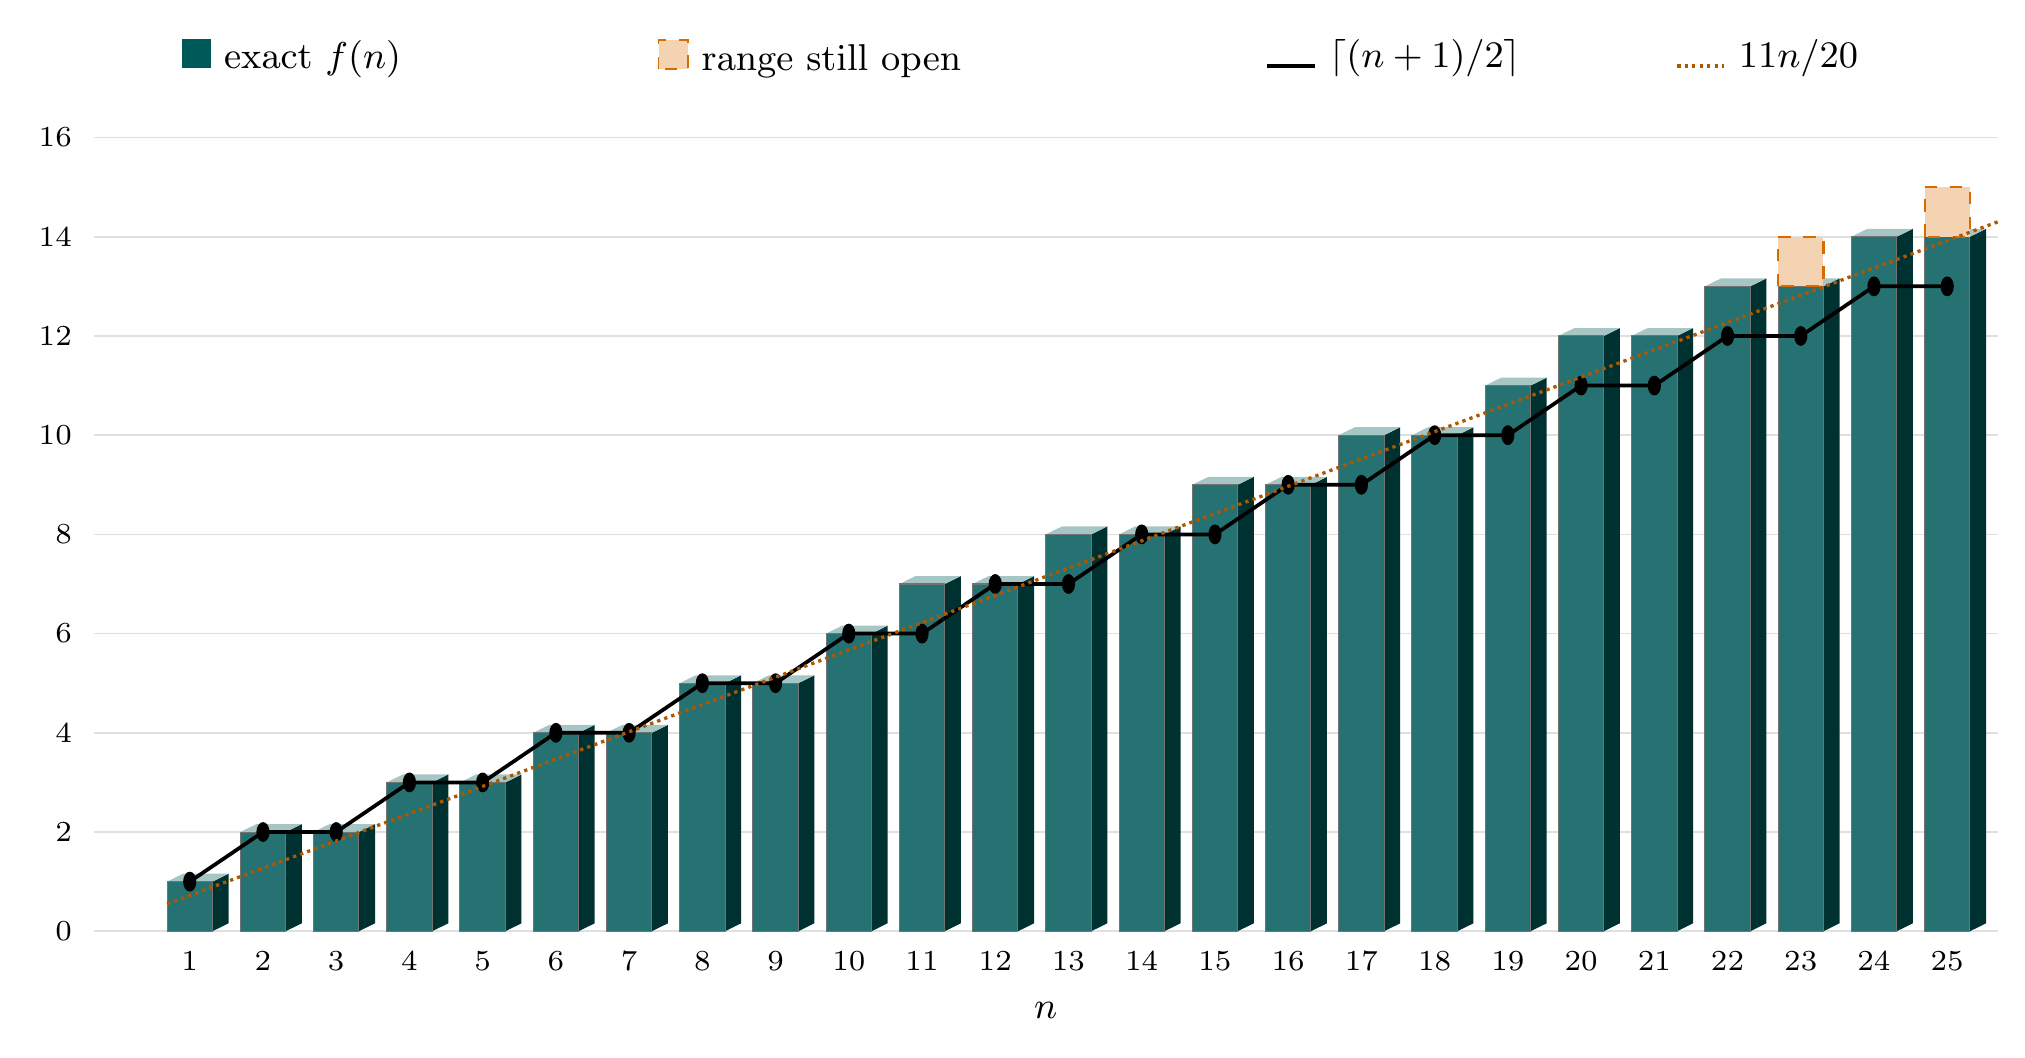
\includegraphics[width=0.93\textwidth]{figures/fig_values.png}
\caption{The values of $f(n)$ for $n\le25$. The bars are exact except at
$n=23$ and $n=25$, where $f(n)$ is one of two values. The solid line is the
chain bound and the dotted line the bound $11n/20$ of
\cite{BMB26v5}.}
\label{fig:values}
\end{figure}

The values are shown in Figure~\ref{fig:values}. The upper bounds in
Theorems~\ref{thm:card} and~\ref{thm:exact} are given by explicit words
(Table~\ref{tab:words}, Figure~\ref{fig:words}); the lower bounds for
$\fc(n)$ and the absence of large monochromatic sublattices under the words
are finite statements, which were checked by computer
(Section~\ref{sec:small}). For $n\le10$ the word $g_n$ attains the chain
bound, so the lower bound there is \eqref{eq:chain}; for the other $n\le24$
the lower bounds for $f(n)$ are those of \cite{BMB26v5}. The value
$f(8)=5$ was stated earlier as an unchecked candidate \cite{Nd26}, and
the bound $f(11)\ge7$, which refutes the equality
$f(n)=\lceil(n+1)/2\rceil$ asked about in the first version of
\cite{BMB26}, was proved in \cite{OR26}; we know of no other exact values
in the literature (searched 14 October 2026).

Two features of the data stand out. First, the best colourings found for
$n\le24$ are all cardinality colourings, and wherever $f(n)$ is known it
equals $\fc(n)$. Second, $\fc(25)=15$ while the best lower bound for
$f(25)$ is $14$; either a better lower bound for $f(25)$ exists or the
optimal colourings stop being cardinality colourings at $n=25$. The same
alternative holds at $n=23$, where $\fc(23)=14$ and $f(23)\ge13$.

\subsection*{Organisation}
Section~\ref{sec:birkhoff} recalls the description of sublattices by
posets. Section~\ref{sec:posets} counts posets by their number of down-sets
and Section~\ref{sec:random} proves Theorem~\ref{thm:random}.
Section~\ref{sec:card} turns cardinality colourings into a problem about
weighted posets, and Section~\ref{sec:small} proves
Theorems~\ref{thm:card} and~\ref{thm:exact}. Section~\ref{sec:questions}
lists open questions. The product-of-chains construction of
Section~\ref{sec:random} and a set-theoretic form of the growth identity of
Lemma~\ref{lem:growth} are also proved in Lean~4 \cite{MU21} with Mathlib
\cite{Mathlib20}.

\subsection*{Notation}
Logarithms are to base $2$ unless a base is written. For a finite poset
$J$, a \emph{down-set} is a subset $D\subseteq J$ such that $y\in D$
whenever $y\le x\in D$, and $d(J)$ is the number of down-sets of $J$. The
\emph{width} of $J$ is the largest size of an antichain. A poset on $[h]$ is
\emph{naturally labelled} if $i<_Jj$ implies $i<j$.

%======================================================================
\section{Sublattices and posets}
\label{sec:birkhoff}

The following is Birkhoff's representation of finite distributive
lattices \cite{Bi37}, written for sublattices of $2^{[n]}$; a form of it is
\cite[Lemma~7.8]{BMB26v5}. We include the short proof because the sizes of
the members are what we need.

\begin{lemma}
\label{lem:birkhoff}
Let $\cL$ be a sublattice of $2^{[n]}$, let $b$ be its least and $t$ its
largest member, and for $x\in t\setminus b$ let $L_x$ be the least member
of $\cL$ that contains $x$. Put $x\preceq y$ if $L_x\subseteq L_y$, let $J$
be the poset of classes of the preorder $\preceq$, and let
$\varphi\colon t\setminus b\to J$ send $x$ to its class. Then
\[
D\ \longmapsto\ b\cup\varphi^{-1}(D)
\]
is a bijection from the down-sets of $J$ onto $\cL$, and $|b\cup
\varphi^{-1}(D)|=|b|+w(D)$, where $w(j)=|\varphi^{-1}(j)|\ge1$ and
$w(D)=\sum_{j\in D}w(j)$. Conversely, for disjoint $b,X\subseteq[n]$, a
finite poset $J$ and a surjection $\varphi\colon X\to J$, the family
$\{b\cup\varphi^{-1}(D)\}$, $D$ a down-set of $J$, is a sublattice with
$d(J)$ members.
\end{lemma}

\begin{proof}
Since $\cL$ is closed under intersection, $L_x$ is the intersection of the
members that contain $x$, and every member contains $b$. If $y\in L_x$,
then $L_x$ is a member containing $y$, so $L_y\subseteq L_x$. Let $A\in\cL$
and $X=A\setminus b$. For $x\in X$ we have $L_x\subseteq A$, so
$A=b\cup\bigcup_{x\in X}L_x$, and $X$ is a union of classes forming a
down-set: if $L_y\subseteq L_x$ and $x\in A$, then $y\in L_y\subseteq A$.
Conversely, if $D$ is a down-set of $J$ and $X=\varphi^{-1}(D)$, then
$B=b\cup\bigcup_{x\in X}L_x$ lies in $\cL$, as a union of members (or
$B=b$ if $D$ is empty), and $B=b\cup X$: every $y\in L_x\setminus b$ with
$x\in X$ has $L_y\subseteq L_x$, so $\varphi(y)\in D$. The two maps are
inverse to each other, which proves the bijection; the sizes are clear.
The converse holds because unions and intersections of down-sets are
down-sets and $\varphi^{-1}$ preserves them.
\end{proof}

A naturally labelled poset on $[h]$ exists in every isomorphism class of
$h$-element posets, by choosing a linear extension. Recording, for each
point of $[n]$, whether it lies in $b$, outside $t$, or in the class
$\varphi(x)\in[h]$, we obtain the following count.

\begin{lemma}
\label{lem:countsub}
Let $P(h,m)$ be the number of naturally labelled posets on $[h]$ with
exactly $m$ down-sets. The number of sublattices of $2^{[n]}$ with exactly
$m\ge2$ members is at most
\[
\sum_{h=1}^{n}(h+2)^{n}\,P(h,m).
\]
\end{lemma}

%======================================================================
\section{Posets with a given number of down-sets}
\label{sec:posets}

Let $J$ be a naturally labelled poset on $[h]$ and let $J_j$ be its
restriction to $[j]$. For $j\in[h]$ let
\[
D_j=\{i<j:\ i<_Jj\},\qquad U_j=[j-1]\setminus D_j,\qquad u_j=d(U_j),
\]
where $U_j$ carries the order induced from $J$. Then $D_j$ is a down-set and
$U_j$ an up-set of $J_{j-1}$, and $J_j$ is determined by $J_{j-1}$ and
$U_j$ (Figure~\ref{fig:growth}).

\begin{lemma}
\label{lem:growth}
$d(J_j)=d(J_{j-1})+u_j$ for every $j$, and hence
$d(J)=1+u_1+\dots+u_h$ with every $u_j\ge1$.
\end{lemma}

\begin{proof}
The down-sets of $J_j$ that do not contain $j$ are the down-sets of
$J_{j-1}$. Those that contain $j$ are the sets $E\cup\{j\}$ with $E$ a
down-set of $J_{j-1}$ containing $D_j$, and $E\mapsto E\setminus D_j$ is a
bijection from these $E$ onto the down-sets of $U_j$: if $F$ is a down-set
of $U_j$, then $F\cup D_j$ is a down-set of $J_{j-1}$, because an element
below a member of $D_j$ lies in $D_j$, and an element below a member of $F$
lies in $D_j$ or in $U_j$, and in the latter case in $F$. The empty poset
has one down-set.
\end{proof}

\begin{figure}[t]
\centering
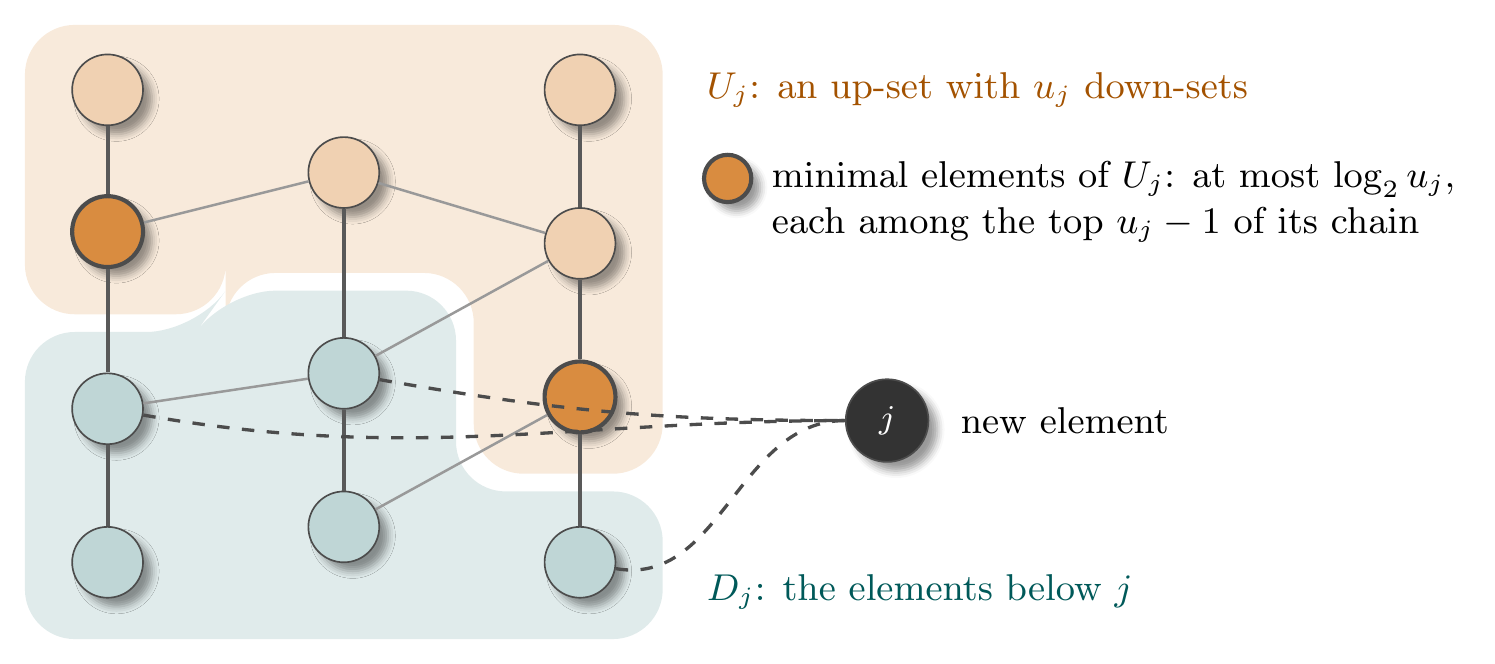
\includegraphics[width=0.86\textwidth]{figures/fig_growth.png}
\caption{Adding the element $j$ to $J_{j-1}$. The down-sets of $J_j$ that
contain $j$ correspond to the down-sets of the up-set $U_j$, and $U_j$ is
determined by its minimal elements, which sit near the tops of the chains
of a chain partition.}
\label{fig:growth}
\end{figure}

Two facts bound the number of choices of $U_j$. If $A$ is an antichain of a
poset $Q$, every subset of $A$ that consists of minimal elements of $Q$ is
a down-set of $Q$; and every antichain of $J$ gives $2^{|A|}$ distinct
down-sets of $J$, namely the down-closures of its subsets, so
\begin{equation}
\label{eq:width}
2^{\width(J)}\ \le\ d(J).
\end{equation}

\begin{lemma}
\label{lem:choices}
Let $w=\max\{1,\width(J_{j-1})\}$. Given $J_{j-1}$ and $u_j=u$, there are
at most $(wu)^{\log u}$ possibilities for $U_j$.
\end{lemma}

\begin{proof}
An up-set is determined by its set $A$ of minimal elements. These form an
antichain of minimal elements of $U_j$, so every subset of $A$ is a
down-set of $U_j$ and $2^{|A|}\le u$. Fix a partition of $J_{j-1}$ into
$w$ chains, which exists by Dilworth's theorem \cite{Di50}. Let $a\in A$
lie in the chain $C$, and let $r$ be the number of elements of $C$ above
$a$. They lie in the up-set $U_j$, so $U_j$ contains a chain $a=c_0<c_1<
\dots<c_r$, whose down-closures in $U_j$ together with $\varnothing$ are
$r+2$ distinct down-sets of $U_j$. Hence $r\le u-2$, and $a$ is one of the
$u-1$ largest elements of its chain. So $A$ is a set of at most $\log u$
elements chosen among at most $N=w(u-1)$ candidates, and the number of
choices is at most $\sum_{i\le\log u}\binom Ni\le(N+1)^{\log u}\le
(wu)^{\log u}$.
\end{proof}

\begin{proposition}
\label{prop:posets}
For $h\ge1$ and $m\ge2$,
\[
\log P(h,m)\ \le\ \log\binom{m-2}{h-1}\ +\ \max\sum_{j=1}^{h}\log u_j\,
\bigl(\log u_j+\log\log m\bigr),
\]
the maximum taken over $u_1,\dots,u_h\ge1$ with $u_1+\dots+u_h=m-1$.
Consequently, for all $\delta,\gamma>0$ there is $n_0$ such that
\[
P(h,m)\ \le\ 2^{\delta m}\qquad\text{whenever } n\ge n_0,\ 1\le h\le n
\text{ and } m\ge\gamma\,n\log n .
\]
\end{proposition}

\begin{proof}
By Lemma~\ref{lem:growth} the sequence $(u_1,\dots,u_h)$ is a composition
of $m-1$ into $h$ positive parts, and there are $\binom{m-2}{h-1}$ of them.
Given the sequence, the poset is built one element at a time, and
Lemma~\ref{lem:choices} bounds the number of choices at step $j$ by
$(wu_j)^{\log u_j}$ with $w\le\max\{1,\log m\}$ by \eqref{eq:width},
because $\width(J_{j-1})\le\width(J)$. This is the first inequality.

For the second, we may assume $m\le2^{h}\le2^{n}$, since a poset on $[h]$
has at most $2^{h}$ down-sets, and that $n$ is so large that $\gamma\log n\ge e$. Write $x=m/h\ge m/n\ge\gamma\log n$.
The function $\psi(y)=(\log(ey))^{2}$ is concave and increasing on
$[1,\infty)$ and $\psi(y)\ge(\log y)^{2}$ there, and $\log$ is concave, so
by Jensen's inequality
\[
\sum_j(\log u_j)^{2}\le h\,\psi(m/h)=m\,\frac{\psi(x)}{x},\qquad
\sum_j\log u_j\le h\log(m/h)=m\,\frac{\log x}{x}.
\]
The functions $\psi(y)/y$ and $(\log y)/y$ both decrease for $y\ge e$,
so that
\[
\frac{\psi(x)}{x}\le\frac{\psi(\gamma\log n)}{\gamma\log n}\longrightarrow0.
\]
For the term with $\log\log m$ we use $\log\log m\le\log n$ and
distinguish two cases. If $m\le n^{3}$, then $\log\log m\le\log(3\log n)$
and
\[
\frac{\log x}{x}\le\frac{\log(\gamma\log n)}{\gamma\log n};
\]
if $m>n^{3}$, then $x>n^{2}$ and $(\log x)/x<2\log n/n^{2}$. In both cases
$\log\log m\cdot(\log x)/x\to0$. Finally,
\[
\log\binom{m-2}{h-1}\le h\log\frac{em}{h}=m\,\frac{\log(ex)}{x},\qquad
\frac{\log(ex)}{x}\le\frac{\log(e\gamma\log n)}{\gamma\log n}\to0 .
\]
All three ratios to $m$ tend to $0$ uniformly in $h\le n$ and
$m\ge\gamma\,n\log n$, which proves the second
statement.
\end{proof}

\begin{remark}
\label{rem:posetcount}
The bound of Proposition~\ref{prop:posets} is far from the number
$2^{h^{2}/4+O(h)}$ of all posets on $[h]$ \cite{KR75}. The point is that
posets on $h\le n$ elements with $m\ge n\log n$ down-sets are thin: their
width is at most $\log m$, and each new element is attached by at most
$\log u_j$ generators near the tops of the chains.
\end{remark}

%======================================================================
\section{Random colourings}
\label{sec:random}

\subsection{The upper bound}
Let $\chi$ be a uniformly random $k$-colouring of $2^{[n]}$, let $\delta>0$
and put $m=\lceil(1+\delta)\,n\log_kn\rceil$. A fixed family of $M$
distinct sets is monochromatic with probability $k^{1-M}$. If some
monochromatic sublattice has at least $m$ members, then some sublattice
with exactly $M\ge m$ members is monochromatic; we do not need to pass to a
sub-sublattice of exactly $m$ members, but sum over all $M\ge m$. By
Lemma~\ref{lem:countsub} and Proposition~\ref{prop:posets}, applied with
$\gamma=1/\log k$ and a constant $\eta>0$ in place of $\delta$ to be chosen,
for large $n$,
\begin{align*}
\Pr[\Lambda(\chi)\ge m]\ &\le\ \sum_{M\ge m}k^{1-M}\sum_{h=1}^{n}(h+2)^{n}
P(h,M)\\
&\le\ \sum_{M\ge m}kn\,(n+2)^{n}\,2^{\eta M}k^{-M}.
\end{align*}
Since $(n+2)^{n}\le e^{2}n^{n}$ and $n\log n=\log k\cdot n\log_kn\le
M\log k/(1+\delta)$ for $M\ge m$, the logarithm of the summand is at most
\[
\log(e^{2}kn)\ -\ M\Bigl(\log k-\eta-\frac{\log k}{1+\delta}\Bigr)
\ =\ \log(e^{2}kn)-cM,
\]
where $c=\log k\cdot\delta/(1+\delta)-\eta$. Taking
$\eta=\log k\cdot\delta/(2+2\delta)$ makes $c>0$, and then
\[
\Pr[\Lambda(\chi)\ge m]\ \le\ \frac{e^{2}kn\,2^{-cm}}{1-2^{-c}}\
\longrightarrow\ 0,
\]
because $m\ge n$. This proves the upper bound of Theorem~\ref{thm:random}
and, since a colouring with $\Lambda(\chi)<m$ exists for large $n$,
Corollary~\ref{cor:upper}.

\subsection{The lower bound}
Let $0<\eps<1$, put $\mu=\lfloor(1-\eps)\log_kn\rfloor$ and assume $n$ is
so large that $\mu\ge1$. Let $Z=\{z_1,\dots,z_{\mu-1}\}$ consist of the
last $\mu-1$ points of $[n]$, let $\cM$ be the chain
$\varnothing\subset\{z_1\}\subset\{z_1,z_2\}\subset\dots\subset Z$ with
$\mu$ members, and let $Y=[n]\setminus Z$. Fix a colour $c$. Call a set
$A\subseteq Y$ \emph{good} if $A\cup S$ has colour $c$ for every
$S\in\cM$. Distinct sets $A$ are tested on disjoint collections of sets
$A\cup S$, since $A=(A\cup S)\cap Y$; hence the events that different sets
are good are independent, each of probability
\[
p=k^{-\mu}\ \ge\ n^{-(1-\eps)} .
\]

We build a chain $A_1\subset A_2\subset\dots$ of good sets with
$|A_i|=i$ greedily. Put $A_0=\varnothing$. At step $i\ge1$ we examine the
$|Y|-i+1$ sets $A_{i-1}\cup\{y\}$ with $y\in Y\setminus A_{i-1}$ and let
$A_i$ be the first good one. Every set examined at step $i$ has size $i$,
so it was not examined before, and its goodness is independent of
everything revealed so far. Hence step $i$ fails with probability
\[
(1-p)^{|Y|-i+1}\ \le\ \exp\bigl(-p(|Y|-i+1)\bigr),
\]
which is at most $\exp(-n^{\eps/2})$ as long as $|Y|-i+1\ge n^{1-\eps/2}$.
By the union bound, with probability at least $1-n\exp(-n^{\eps/2})$ the
procedure produces good sets $A_1\subset\dots\subset A_h$ with
$h\ge|Y|-n^{1-\eps/2}\ge n-\log_kn-n^{1-\eps/2}$.

The family $\{A_i\cup S:\ 1\le i\le h,\ S\in\cM\}$ is a sublattice, since
for chains in disjoint ground sets
\begin{align*}
(A\cup S)\cup(A'\cup S')&=(A\cup A')\cup(S\cup S'),\\
(A\cup S)\cap(A'\cup S')&=(A\cap A')\cup(S\cap S'),
\end{align*}
and the union and the intersection of two members of a chain is one of
them. Its members are distinct, again because $A=(A\cup S)\cap Y$, and all
have colour $c$. It has
\[
h\mu\ \ge\ \bigl(n-\log_kn-n^{1-\eps/2}\bigr)\bigl((1-\eps)\log_kn-1\bigr)
\ \ge\ (1-2\eps)\,n\log_kn
\]
members for large $n$. Applying this to each of the $k$ colours and
replacing $\eps$ by $\eps/2$ proves the lower bound of
Theorem~\ref{thm:random}, including the statement for every colour.
\qed

\begin{figure}[t]
\centering
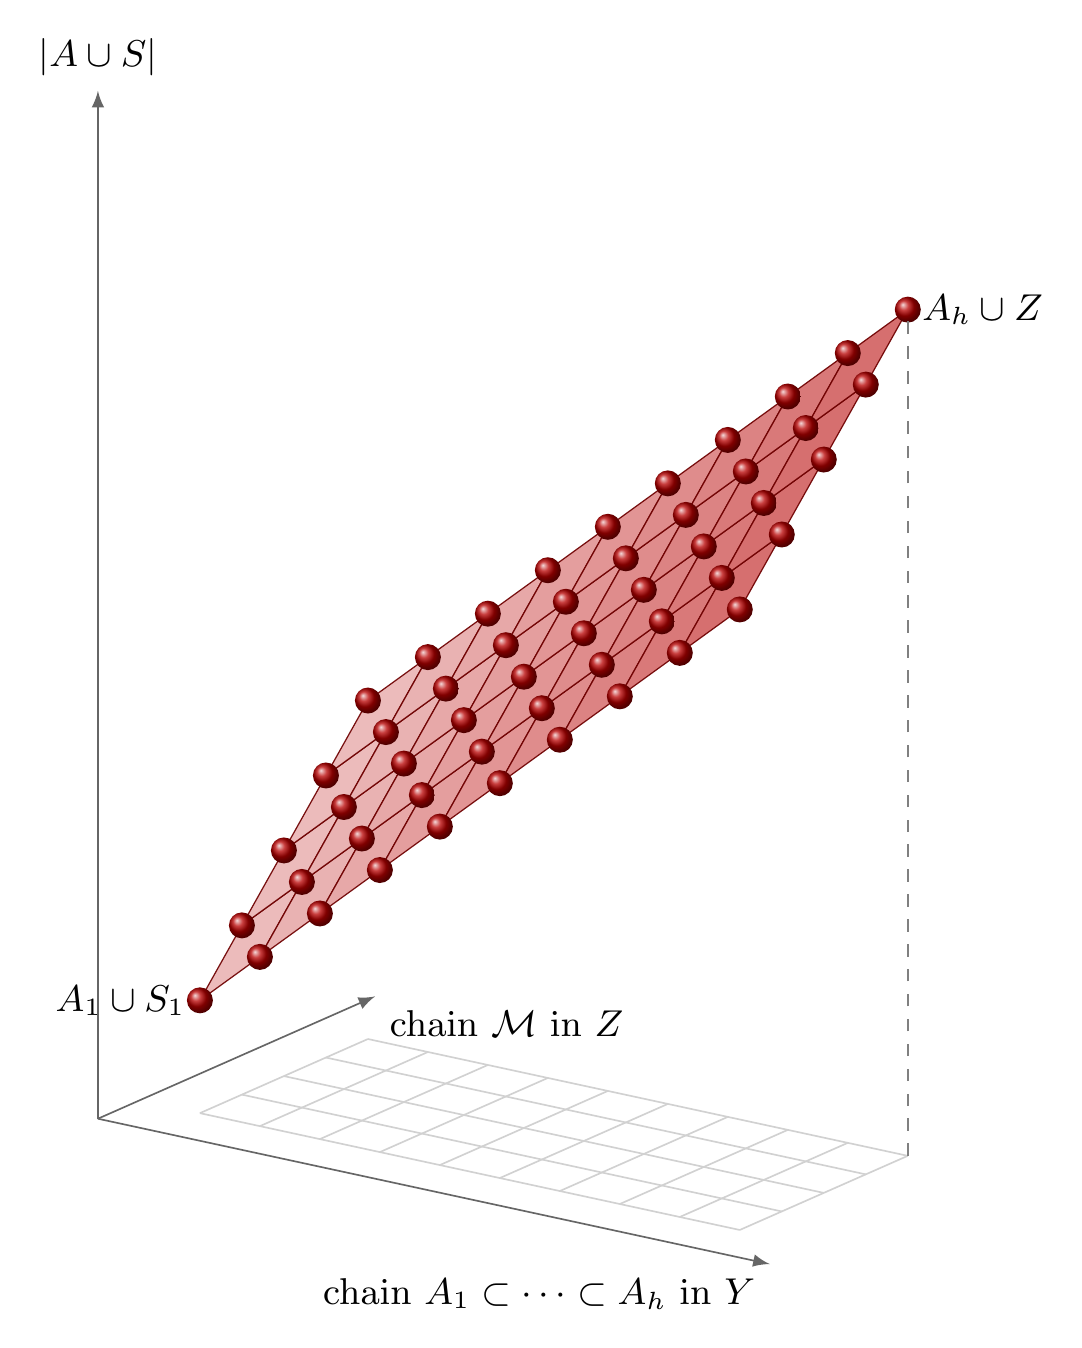
\includegraphics[width=0.56\textwidth]{figures/fig_product.png}
\caption{The monochromatic sublattice built in the lower bound: a
greedy chain of good sets in $Y$ times a short chain in $Z$. Its members
form a grid, drawn with height equal to the size of each set.}
\label{fig:product}
\end{figure}

\begin{remark}
\label{rem:randomshape}
The two halves of the proof explain the constant. A sublattice with $m$
members in which every set is a product of a long chain and a chain of
length $\mu$ uses about $n$ independent tests, each of probability
$k^{-\mu}$; the long chain is available only while $k^{\mu}\le n$. The
counting bound says that no other shape does better to first order, since
there are only $(n+2)^{n}2^{o(m)}=k^{(1+o(1))\,n\log_kn}$ sublattices with
$m\approx n\log_kn$ members.
\end{remark}

%======================================================================
\section{Colourings by cardinality}
\label{sec:card}

Let $g\colon\{0,1,\dots,n\}\to\{\w R,\w B\}$ and colour $A\subseteq[n]$
by $g(|A|)$. For a colour $c$ let $S_c=g^{-1}(c)$. A \emph{weighted poset}
is a finite poset $J$ with a weight $w\colon J\to\{1,2,\dots\}$, and a
\emph{placement} of it in $\{0,\dots,n\}$ is an integer $\beta\ge0$ with
$\beta+w(J)\le n$. By Lemma~\ref{lem:birkhoff} the sublattices of $2^{[n]}$
are, up to the choice of the points, the placed weighted posets, and a
member corresponding to a down-set $D$ has size $\beta+w(D)$. Hence:

\begin{lemma}
\label{lem:weighted}
The largest monochromatic sublattice of colour $c$ under $g$ has as many
members as the largest $d(J)$ over placed weighted posets $(J,w,\beta)$
with $\beta+w(D)\in S_c$ for every down-set $D$ of $J$.
\end{lemma}

We call such a placed weighted poset \emph{$c$-monochromatic}. In
Figure~\ref{fig:downsets} the poset $a\parallel(b<c)$ with weights
$1,3,5$ and $\beta=0$ has down-set sums $0,1,3,4,8,9$, all red for the word
$g_{10}$ of Table~\ref{tab:words}; this red sublattice has six members,
which is the largest possible for that word.

\begin{figure}[t]
\centering
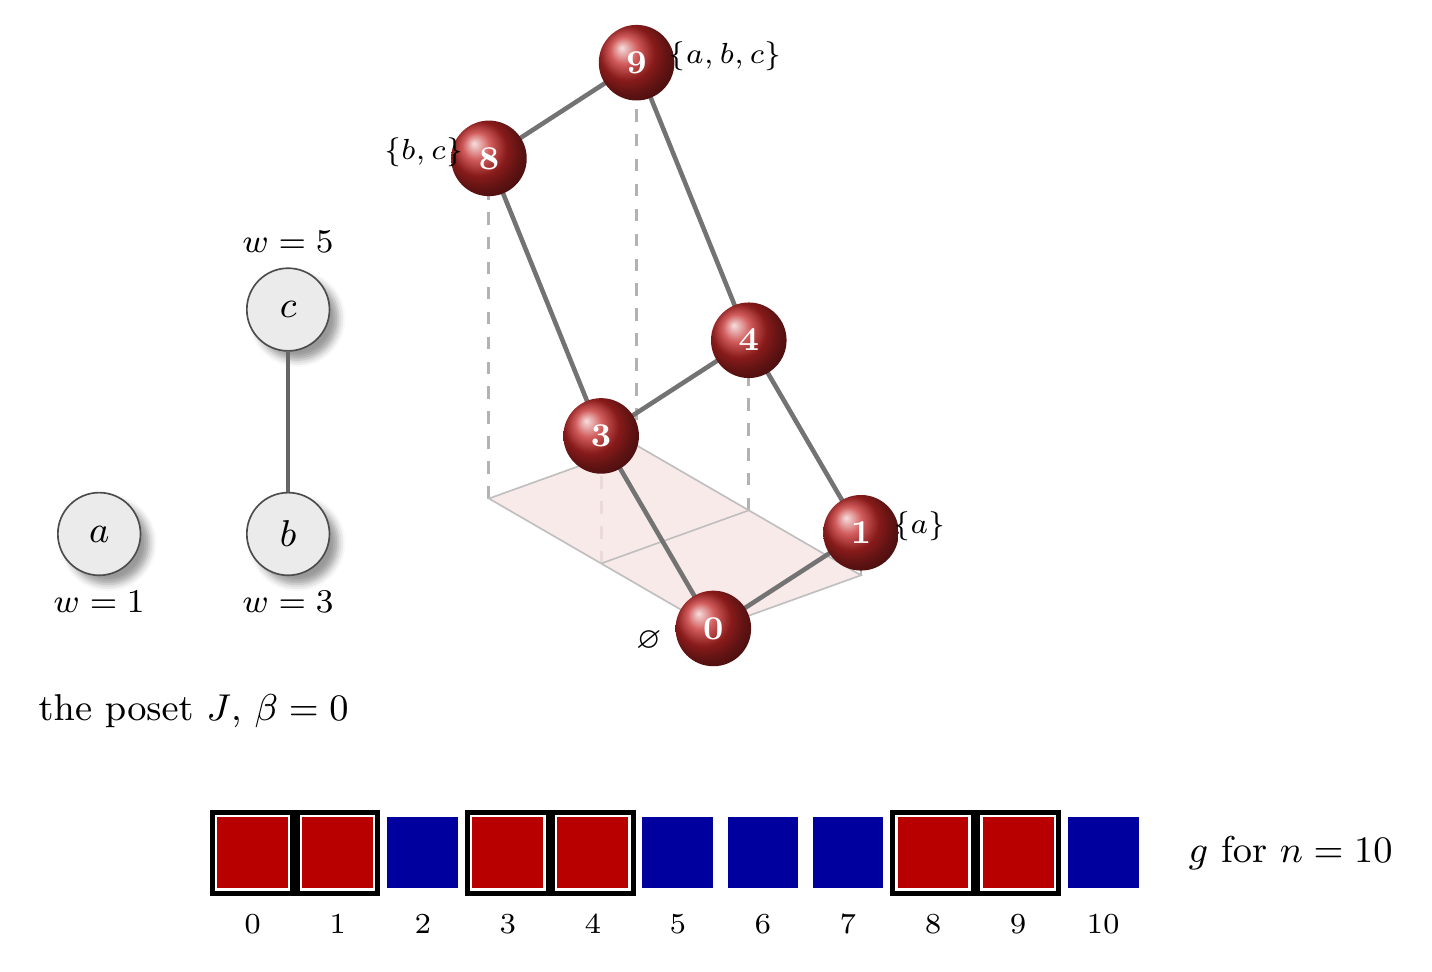
\includegraphics[width=0.8\textwidth]{figures/fig_downsets.png}
\caption{A weighted poset, its lattice of down-sets with the down-set sums,
and the word $g_{10}$, which is red at all six sums.}
\label{fig:downsets}
\end{figure}

Two properties make the search over weighted posets finite and complete.

\begin{lemma}
\label{lem:prefix}
Let $(J,w,\beta)$ be $c$-monochromatic, with $J$ naturally labelled on
$[h]$. Then each restriction $(J_j,w|_{[j]},\beta)$ is $c$-monochromatic,
and if $d(J)\ge K$ there is $j$ with $K\le d(J_j)\le K-1+u_j$.
\end{lemma}

\begin{proof}
A down-set of $J_j$ is a down-set of $J$ with the same sum. The numbers
$d(J_j)$ increase from $d(J_0)=1$ to $d(J)$ in steps $u_j$ by
Lemma~\ref{lem:growth}; take the first $j$ with $d(J_j)\ge K$.
\end{proof}

So to decide whether $g$ has a $c$-monochromatic sublattice with $K$
members it suffices to grow naturally labelled weighted posets one element
at a time, attaching the new element above a down-set $D_j$ of the current
poset with a weight $w_j\ge1$, keeping only those placements in which all
down-set sums lie in $S_c$, and stopping as soon as $K$ down-sets are
reached. Each attachment adds the sums $\beta+w(E)+w_j$ for the down-sets
$E\supseteq D_j$, so the condition can be checked incrementally. The dual
procedure, which adds minimal elements below an up-set and keeps the top
value $\beta+w(J)$ fixed, gives a second, independent decision procedure.

Arithmetic progressions in $S_c$ give Boolean cubes: if $g$ is constant on
$a,a+e,\dots,a+(p-1)e$, then $g$ has a monochromatic sublattice with
$2^{p-1}$ members \cite[Proposition~6.2]{BMB26v5}. Thus a word without
large monochromatic sublattices has no long monochromatic progressions,
and the words of Table~\ref{tab:words} have none of length five; for
$n\ge16$ their longest monochromatic progressions have length four.

%======================================================================
\section{Small values}
\label{sec:small}

\begin{table}[t]
\centering
\scriptsize
\setlength{\tabcolsep}{3pt}
\renewcommand{\arraystretch}{1.08}
\begin{tabular}{@{}rcl@{\quad}rcl@{}}
\toprule
$n$ & $\fc(n)$ & word $g_n$ & $n$ & $\fc(n)$ & word $g_n$\\
\midrule
1 & 1 & \w{RB} & 14 & 8 & \w{RBRRBBBRRBBRBRR}\\
2 & 2 & \w{RRB} & 15 & 9 & \w{RBBRBRRBBBRBRRRB}\\
3 & 2 & \w{RRBB} & 16 & 9 & \w{RRBRBBRRBBBRBRRBR}\\
4 & 3 & \w{RRBRB} & 17 & 10 & \w{BRBBRRBBBRBRRBBRRR}\\
5 & 3 & \w{RRBRBB} & 18 & 10 & \w{RRBBRRBRBBBRRBBRBRR}\\
6 & 4 & \w{BBRRBRR} & 19 & 11 & \w{BRBBRRRBBRBRRBBBRRBR}\\
7 & 4 & \w{BBRRBBRR} & 20 & 12 & \w{RRBBRBBBRRBRBBRRRBBRR}\\
8 & 5 & \w{RBBBRRBRR} & 21 & 12 & \w{BBRRBBRBRRRBBBRBRRBBRR}\\
9 & 5 & \w{BBRBRRBBRR} & 22 & 13 & \w{BRRBRBBRRRBBRRBRBBBRRBR}\\
10 & 6 & \w{RRBRRBBBRRB} & 23 & 14 & \w{BBRRBRBBBRRBRBBRRRBBRRBR}\\
11 & 7 & \w{RRRBRRBBBRBB} & 24 & 14 & \w{RRBBRBRRBBBRBRRBBRBRBRRBR}\\
12 & 7 & \w{RRBBBRRBRBBRR} & 25 & 15 & \w{BRBBRRBBBRBRRBRRRBBBRBRRBR}\\
13 & 8 & \w{RBBBRRBRBBRRRB} &  &  & \\
\bottomrule
\end{tabular}
\medskip
\caption{Optimal cardinality colourings. Under $g_n$ every monochromatic
sublattice of $2^{[n]}$ has at most $\fc(n)$ members.}
\label{tab:words}
\end{table}

\begin{figure}[t]
\centering
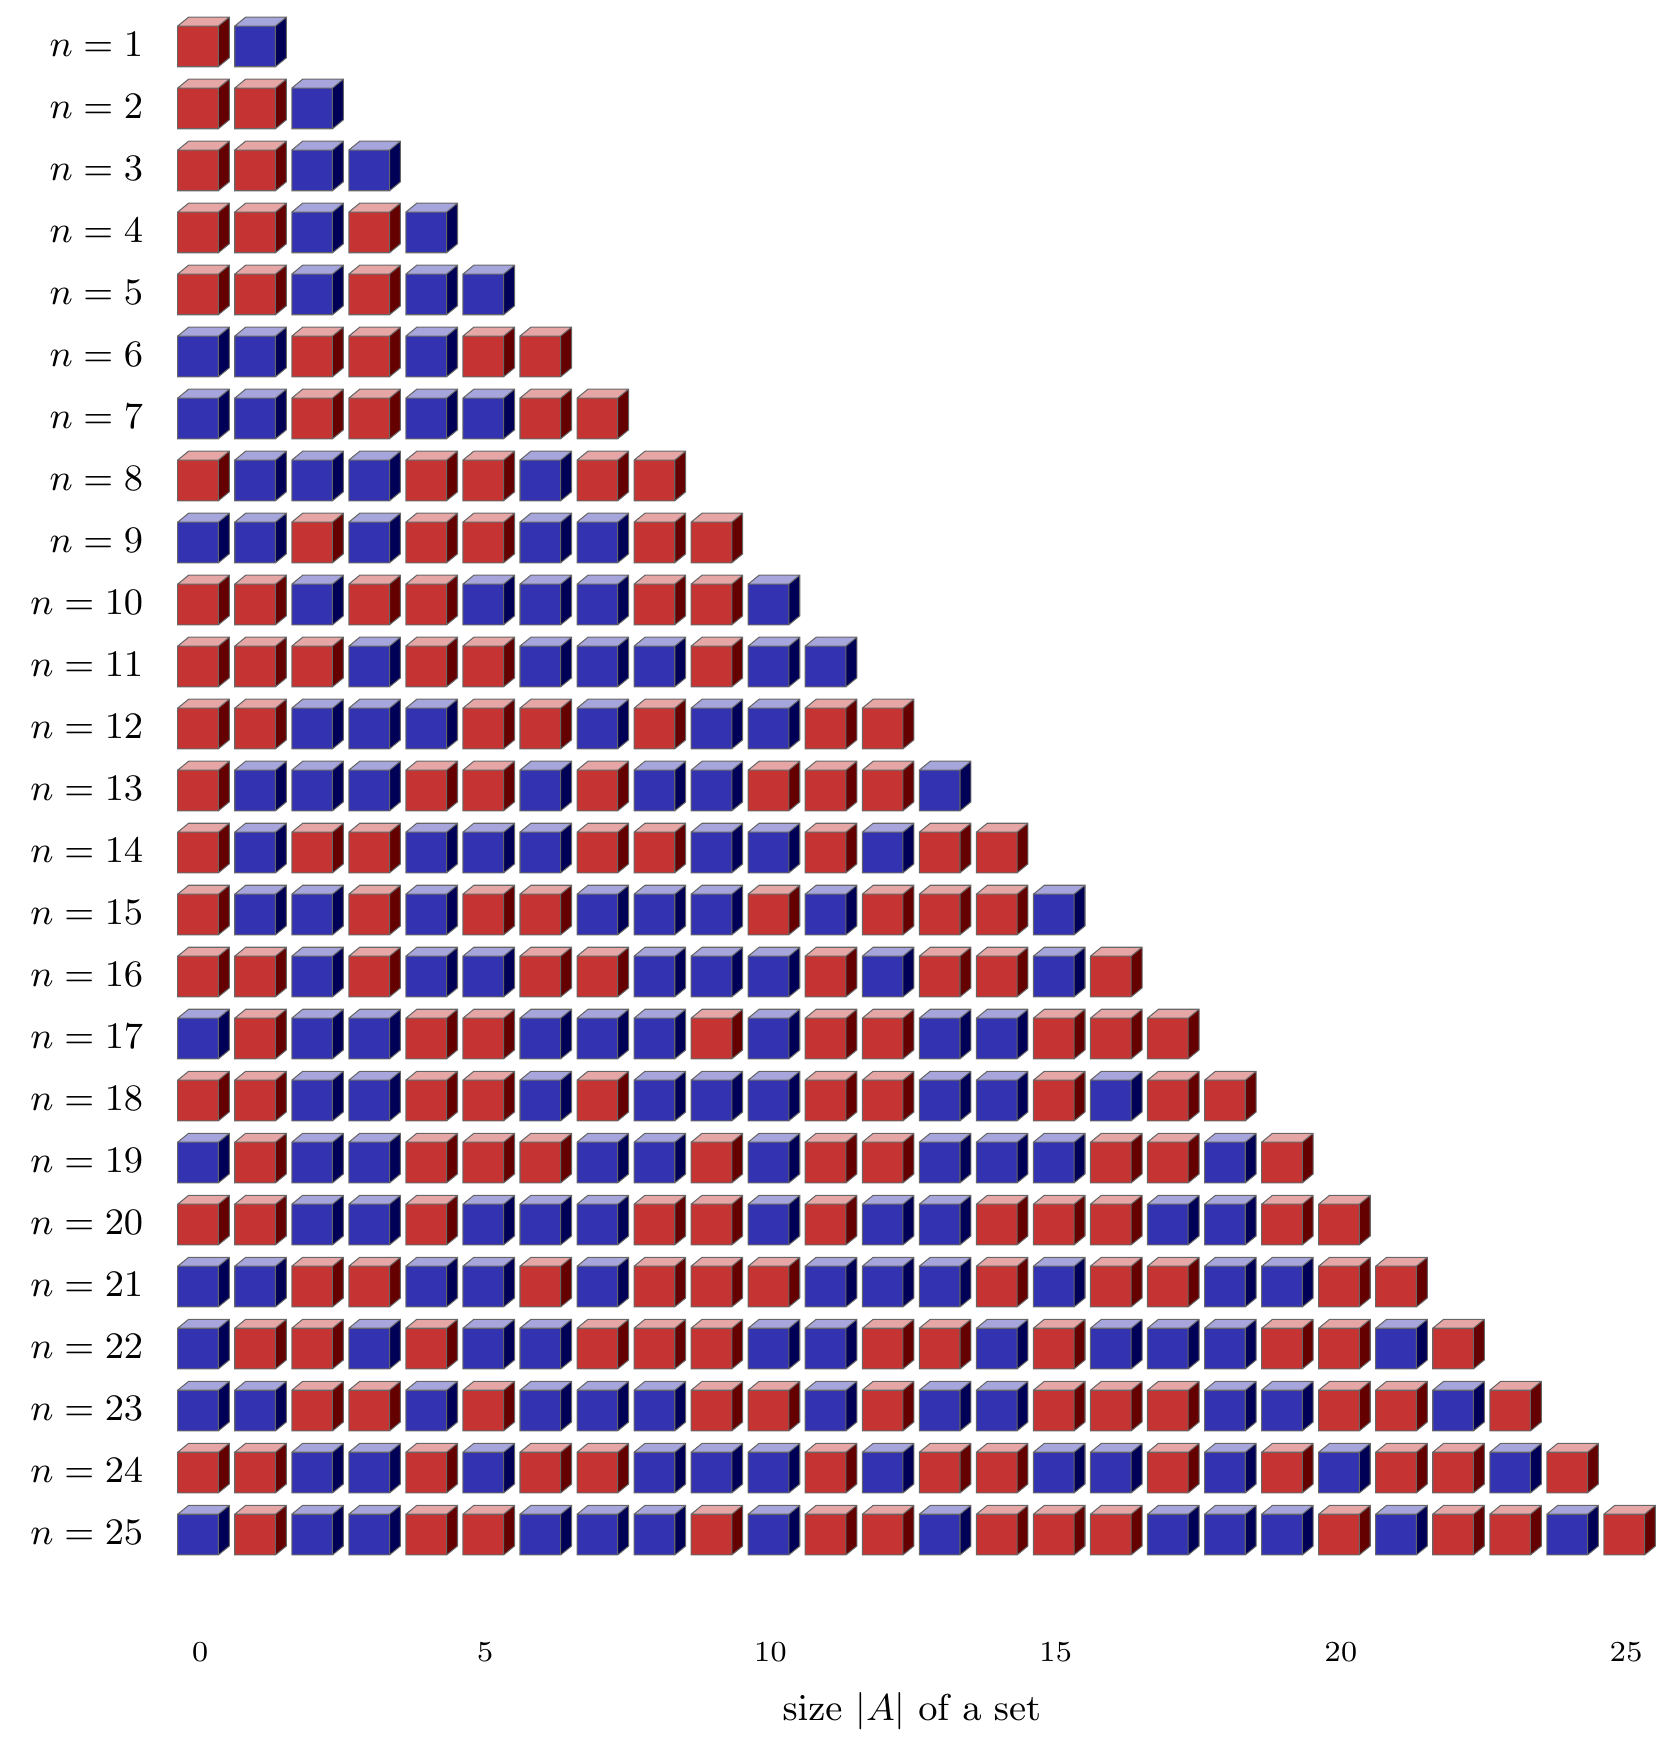
\includegraphics[width=0.74\textwidth]{figures/fig_words.png}
\caption{The words $g_n$ of Table~\ref{tab:words}; the cell in column $i$
of row $n$ is the colour of the sets of size $i$.}
\label{fig:words}
\end{figure}

\begin{lemma}
\label{lem:words}
For $1\le n\le25$, every monochromatic sublattice of $2^{[n]}$ under the
cardinality colouring $g_n$ of Table~\ref{tab:words} has at most $\fc(n)$
members, with $\fc(n)$ as in Table~\ref{tab:words}.
\end{lemma}

\begin{proof}
By Lemma~\ref{lem:weighted} it suffices to show that for each colour $c$
there is no $c$-monochromatic placed weighted poset with $\fc(n)+1$
down-sets, and by Lemma~\ref{lem:prefix} the search described after it
decides this. Both the search and its dual were run for every $n\le25$ and
both colours, and both found no such poset.
\end{proof}

\begin{lemma}
\label{lem:cardlower}
For $1\le n\le25$, every word $g\colon\{0,\dots,n\}\to\{\w R,\w B\}$ has a
monochromatic sublattice with at least $\fc(n)$ members, with $\fc(n)$ as
in Table~\ref{tab:words}.
\end{lemma}

\begin{proof}
For $n\le10$ this is the chain bound \eqref{eq:chain}. For the other $n$
we produced a list $\mathcal{W}_n$ of placed weighted posets, each with at
least $\fc(n)$ down-sets, and checked that every word is constant on the
set of down-set sums of some member of $\mathcal{W}_n$; by
Lemma~\ref{lem:weighted} this proves the claim. Each member of
$\mathcal{W}_n$ is a pair of clauses of a propositional formula in the
variables $g(0),\dots,g(n)$, saying that $g$ is not constant on its set of
sums, and the claim is that the formula is unsatisfiable. The lists were
found by alternating a satisfiability solver, which proposes a word, with
the search of Section~\ref{sec:card}, which returns a monochromatic poset
for that word. Each certificate was then checked independently: the
down-sets of every poset in $\mathcal{W}_n$ were recomputed from scratch,
and the unsatisfiability of the formula was confirmed by two different
solvers. The lists have between $288$ (for $n=11$) and $49{,}078$ (for
$n=25$) members.
\end{proof}

\begin{proof}[Proof of Theorem~\ref{thm:card}]
Lemmas~\ref{lem:words} and~\ref{lem:cardlower}.
\end{proof}

\begin{proof}[Proof of Theorem~\ref{thm:exact}]
The upper bounds $f(n)\le\fc(n)$ hold because cardinality colourings are
colourings. For the lower bounds let $n+1=20q+r$ with $0\le r\le19$ and
$e=[r\ge12]$, and $q'=\lfloor(n+1)/12\rfloor$. By
\cite[Theorems~1.4 and~7.6]{BMB26v5},
\[
f(n)\ \ge\ \max\Bigl\{\Bigl\lceil\frac{n+1+q'}{2}\Bigr\rceil,\
\Bigl\lceil\frac{n+1+2q+e}{2}\Bigr\rceil\Bigr\}.
\]
For $n\le10$ this is $\lceil(n+1)/2\rceil=\fc(n)$. For odd $n$ with
$11\le n\le21$ the first term is $(n+3)/2=\fc(n)$; for
$n\in\{12,14,16,18\}$ it is $(n+2)/2=\fc(n)$. For $n=20$ and $n=22$ the
second term gives $12$ and $13$, and for $n=24$ the first gives $14$; these
equal $\fc(n)$. For $n=23$ and $n=25$ both terms are at most $13$ and $14$
respectively.
\end{proof}

The values $f(20)=12$ and $f(22)=13$ depend on the window lemma of
\cite[Lemma~7.7]{BMB26v5}, which is proved by a finite computation; all
other lower bounds in Theorem~\ref{thm:exact} are proved by hand in
\cite{BMB26v5}.

%======================================================================
\section{Questions}
\label{sec:questions}

Theorem~\ref{thm:random} locates the random colouring precisely, and
\eqref{eq:known} leaves a factor of order $\log n$ for $f(n)$.

\begin{question}
\label{q:card}
Is $\fc(n)=O(n)$? If so, is $\fc(n)/n$ convergent?
\end{question}

For $10\le n\le25$ the ratio $\fc(n)/(n+1)$ lies between $1/2$ and $0.59$.
A positive answer would give $f(n)=O(n)$, answering
\cite[Question~9.3]{BMB26v5}. Good words must avoid long monochromatic
progressions, since a progression of length $p$ gives a sublattice with
$2^{p-1}$ members, and more generally they must avoid the down-set sums of
every weighted poset with many down-sets.

\begin{question}
\label{q:23}
Is $f(23)=13$ or $14$, and is $f(25)=14$ or $15$? Is there any $n$ with
$f(n)<\fc(n)$?
\end{question}

\begin{question}
\label{q:k}
Is $f_k(n)=(1+o(1))\,(n+1)/k$ for $k\ge3$, or does $f_k(n)/n$ stay above
$1/k$ by a constant, as \eqref{eq:known} shows for $k=2$?
\end{question}

\section*{Data availability}

The words of Table~\ref{tab:words}, the certificates of
Lemma~\ref{lem:cardlower}, the programs that produce and check them (in C++
and Python), and the Lean formalisation are available at
\url{\codeurl}. The programs
and the Lean formalisation were written with the assistance of Claude Code
(Anthropic).

\begin{thebibliography}{BMB26b}
\raggedright

\bibitem[BMB26a]{BMB26}
D.~Bhattacharjee, P.~Mandal and U.~Bhattacharya,
\emph{Resolving Erd\H{o}s--Ulam monochromatic union-closed family
conjectures}, preprint (2026),
\href{https://arxiv.org/abs/2610.02833}{arXiv:2610.02833}.

\bibitem[BMB26b]{BMB26v5}
D.~Bhattacharjee, P.~Mandal and U.~Bhattacharya,
\emph{Resolving Erd\H{o}s--Ulam monochromatic union-closed family
conjectures}, version~5 with Lean formalisation, Zenodo (2026),
\href{https://doi.org/10.5281/zenodo.23374973}{doi:10.5281/zenodo.23374973}.

\bibitem[Bi37]{Bi37}
G.~Birkhoff,
\emph{Rings of sets},
Duke Math. J. \textbf{3} (1937), no.~3, 443--454.
\href{https://doi.org/10.1215/S0012-7094-37-00334-X}{doi:10.1215/S0012-7094-37-00334-X}

\bibitem[Bl26]{Bl26}
T.~F. Bloom,
\emph{Erd\H{o}s Problem \#1183},
\url{https://www.erdosproblems.com/1183}, accessed 14 October 2026.

\bibitem[Ch26]{Ch26}
P.~Chojecki,
\emph{Monochromatic union-closed and lattice subfamilies of the Boolean
lattice}, preprint, 18 March 2026,
\url{https://www.ulam.ai/research/erdos1183.pdf}.

\bibitem[Di50]{Di50}
R.~P. Dilworth,
\emph{A decomposition theorem for partially ordered sets},
Ann. of Math. (2) \textbf{51} (1950), no.~1, 161--166.
\href{https://doi.org/10.2307/1969503}{doi:10.2307/1969503}

\bibitem[KR75]{KR75}
D.~J. Kleitman and B.~L. Rothschild,
\emph{Asymptotic enumeration of partial orders on a finite set},
Trans. Amer. Math. Soc. \textbf{205} (1975), 205--220.
\href{https://doi.org/10.1090/S0002-9947-1975-0369090-9}{doi:10.1090/S0002-9947-1975-0369090-9}

\bibitem[Mat20]{Mathlib20}
The mathlib Community,
\emph{The Lean mathematical library},
in: Proceedings of the 9th ACM SIGPLAN International Conference on
Certified Programs and Proofs, CPP 2020, ACM, New York, 2020, 367--381.
\href{https://doi.org/10.1145/3372885.3373824}{doi:10.1145/3372885.3373824}

\bibitem[MU21]{MU21}
L.~de~Moura and S.~Ullrich,
\emph{The Lean~4 theorem prover and programming language},
in: Automated Deduction, CADE~28,
Lecture Notes in Comput. Sci. 12699, Springer, Cham, 2021, 625--635.
\href{https://doi.org/10.1007/978-3-030-79876-5_37}{doi:10.1007/978-3-030-79876-5\_37}

\bibitem[Nd26]{Nd26}
ndrorchestration,
\emph{Stage Erd\H{o}s \#1183 $f(8)=5$ and $F(8)\le8$ candidate
verification}, GitHub pull request, 15 September 2026,
\url{https://github.com/ndrorchestration/ndrorchestration/pull/19}.

\bibitem[OR26]{OR26}
The Omega Institute,
\emph{Refute $f(n)=\lceil(n+1)/2\rceil$ via $f(11)\ge7$}, trureturing
issue \#14535, 8--9 October 2026,
\url{https://github.com/the-omega-institute/trureturing/issues/14535}.

\end{thebibliography}

\end{document}
